\documentclass[3p]{elsarticle}
\usepackage{tipa}
\usepackage{amsmath}%math
\usepackage{amsthm}%proof
\usepackage{xcolor}%color
\usepackage{bm}
\usepackage{graphicx}
\usepackage{booktabs}
\usepackage{textcomp}
\usepackage[colorlinks,linkcolor=black,anchorcolor=black,citecolor=black]{hyperref}
\usepackage{amsfonts,amssymb}
\usepackage{multirow}
\usepackage[titletoc]{appendix}
\usepackage{float}


\theoremstyle{plain}
\newtheorem{assumption}{Assumption}
\newtheorem{mydef}{Definition}
\newtheorem{mylem}{Lemma}
\newtheorem{myrem}{Remark}
\newtheorem{thm}{Theorem}
\begin{document}
%\begin{twocolumn}
\begin{frontmatter}
\title{Adaptive Sliding Mode Control of Tethered Satellite Flight with Input Saturation}
\author{Zhiqiang Ma}
\author{Guanghui Sun\corref{cor1}}
\ead{guanghuisun@hit.edu.cn}
%\ead{mazhiqianghit@163.com}
\cortext[cor1]{Corresponding author}
\address{Research Institute of Intelligent Control and Systems, Harbin Institute of Technology, Harbin 150001, China}
\begin{abstract}
This paper proposes  a  novel adaptive sliding mode control for the attitude regulation of the multi-satellite inline tethered system, where the input saturation is taken into account. The underactuated governing equations for the attitude dynamics of the three-satellite inline tethered system are derived firstly by utilizing Lagrangian mechanics theory. Considering the fact that the attitude of the central satellite can be adjusted by using the simple exponential stabilization scheme, the decoupling of the central satellite and the terminal ones is presented, and in addition, the new adaptive sliding mode control law is applied to stabilize the attitude dynamics of the two terminal satellites based on the synchronization and partial contraction theory. In the adaptive sliding mode control design, the input is modeled as saturated input due to the fact that the flywheel torque is bounded, and meanwhile, an adaptive update rate is introduced to eliminate the effect of the saturated input and the external perturbation. The proposed control scheme can be applied on the two-satellite system to achieve fixed-point rotation. The numerical results valid the effectiveness of the proposed method.
\end{abstract}
\begin{keyword}
Multi-satellite tethered system;  Adaptive Sliding mode;  Input saturation; Satellite attitude adjusting
\end{keyword}
\end{frontmatter}
\section{Introduction}
Space tethered satellite (STS) systems consist of the orbiting satellites connected by long thin space tethers. Since the conception of the tethered satellite system was addressed in 1960s, many space institutes have implemented a significant number orbital and suborbital experiments, such as TSS-1R, SEDS, MAST, YES2~\cite{williams2012review}, to verify feasibility for the STS studies developed from 1970s to 1980s. Among other things, the STS systems have been ideally qualified for various missions in the space environment, such as the electrodynamic propulsion application~\cite{lanoix2005effect}, deorbiting defunct satellites~\cite{khan2014analysis}, the space tug~\cite{wen2016constrained} and the space elevator~\cite{kojima2015mission}.\par
In recent years, many investigations have been carried out about control law designs and formation flights of the STS systems, providing some effective solutions to the attitude stabilization and flight formations~\cite{zhu2015dynamic,hallaj2015tethered,alary2015dynamics,wang2015coordinated}. For the attitude stability of the STS system, as the simplest formation control strategy, the steerable thruster-based control is used extensively~\cite{aslanov2013dynamics,jasper2014input,jasper2014tethered,aslanov2014dynamics}. However, one should take into account the fact that the availability and consumption of the fuel restricts the work of actuators directly, leading the control to be short-term~\cite{chung2008propellant1}, and moreover, in the traditional thruster-based control schemes, there exists a fatal impact of the jet propulsive working medium on the sensors and the neighbour satellites~\cite{hallaj2015tethered}.\par
To alleviate these concerns of the thruster-based control, some alternative unpure thruster-based schemes for formation flight of the STS systems have been proposed. Miller addressed the concept of electromagnetic formation flying (EMFF), in which the high temperature superconducting technology was utilized for the satellite attitude regulation indirectly~\cite{miller2010control}. Some researches using different control schemes followed to achieve EMFF ~\cite{zhang2014adaptive,huang2015lmi}. Yang investigated the three-inline satellite array, in which the participating satellites were equipped with the reaction wheels and the thrusters, and hence the linear force and torque cooperated to stabilize the attitude of the satellites~\cite{yang2015decentralized}. Natarajan and Schaub combined the Coulomb forces with conventional thrust forces to obtain a control scheme with the Coulomb forces predominating, and investigated the stability of the two-craft formation about various equilibrium configurations~\cite{natarajan2009hybrid}. Among the mentioned actuators, for canceling the drawback of the thrusters in the attitude regulation control, the flywheel as a inter-force actuator has been paid attention to ~\cite{pizarro2008dynamics}. Comparing to the thruster-based scheme, the solar sails providing the power for the flywheels achieves a long-term attitude control for the satellites of the STS system, and furthermore the contamination to the sensitive sensors does not occur. However, without the thrusters forces acting in the attitude regulation, the pure flywheel torque control causes the attitude dynamics underactuated adversely, i.e., Chung et al. introduced the concept of the underactuated multi-satellite inline system, and proposed the underactuated control scheme for the compound pendulum dynamics of the STS system~\cite{chung2008propellant1}.\par
Besides actuator selection, the effective control scheme and the formation type are both important components of the STS system. In recent years, many researchers have strived to investigate the motion dynamics of the multi-satellite inline formation, and there have existed a sort of sophisticated linear control schemes. Chung et al. exploited geometric symmetries to get the reduction dynamics, and investigated the decentralized linear control method for the flight tailored toward the SPECS mission~\cite{chung2007nonlinear}. They also developed a gain-scheduling linear control law adjusting the attitude of the multiple-satellite system without any thruster forces~\cite{chung2008propellant1}. Yang et al. investigated the decentralized fault tolerance control scheme for the attitude of the satellites in the three-inline array around the equilibrium point~\cite{yang2015decentralized}. In the aspect of nonlinear control, Chung et al. presented a backstepping control design for the multi-satellite system after reducing the model into the strict-feedback cascade normal form~\cite{chung2008propellant2}. Zhao et al. applied gauss pseudospectral method to multi-objective trajectory optimization for two spacecrafts~\cite{zhao2014gauss}. Among the previous control systems, all the inputs are regarded as unsaturated, however, in the realistic application the input saturation frequently does occur. Furthermore, the saturation often leads controllers to no longer ensure the performance of regulation objective~\cite{zavala2007natural}. The existence of the input saturation, which usually stems from the physical mechanics and the energy dissipation, usually leads to the fatal differential between the desired control signal and the actual output effort of the actuator, and consequently it is a potential source of the corruption~\cite{Hu2009Robust}. In order to resist the effect of the saturation, some saturated control schemes have been proposed, i.e., Bo{\v{s}}kovi{\'{c}} et al. proposed global stable control algorithms with variable structure philosophy presence of control input saturation~\cite{bovskovic2001robust}; Tsiotras and Luo decoupled the general motion dynamics into two rotations, and proposed a feedback control scheme to regulate the system to track a specified state in the inertial space~\cite{tsiotras2000control}; Grimm et al.~\cite{grimm2003antiwindup}, Xu and Lam~\cite{xu2001robust} paid more attention to the linear systems with the bounded input. Considering the above mentioned technologies, introducing the saturated inputs into the control systems is complicate but meaningful for both the theory studies and the engineering applications.\par
In this paper, a novel adaptive sliding mode control scheme is proposed for the three-satellite inline array and the two-satellite system. This work takes into consideration the characteristics of the coupling input saturation in the control system design, and the linear force is absent in the attitude regulation of the satellite. The remainder of the paper is organized as follows. In Section \ref{sec:mm}, the mathematical model for the flight of three-satellite inline array is presented, and a novel MHSM scheme for the stability of the attitude dynamics is proposed, with emphasis on the solution of the input saturation in Section \ref{sec:SMC}. In Section \ref{sec:SMC2}, the attitude dynamics of two-satellite system is investigated, and applying MHSM scheme to stabilize the attitude dynamics motion is exhibited. Finally the numerical simulation is illustrated to validate the above mentioned control design in Section \ref{sec:sm}.
\section{Mathematical Model For Three-satellite Inline Array}\label{sec:mm}
\begin{figure}
\centering
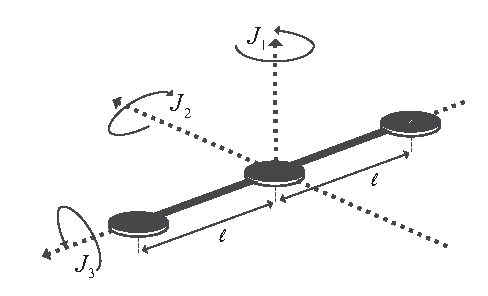
\includegraphics[width=7.68cm,height=4.42cm]{2nd_3satellite.eps}
\caption{Schematic representation of three-satellite inline array}
\label{fig:3satellite}
\end{figure}
The schematic representation of the three-satellite inline array is present in Figure \ref{fig:3satellite}, and the simplified Euler's rotational equations of the motion for the system follows
\begin{align}
\begin{bmatrix}
J_1 &0  &0\\
0   &J_2&0\\
0   &0  &J_3
\end{bmatrix}\begin{pmatrix}
\dot{\omega}_1\\
\dot{\omega}_2\\
\dot{\omega}_3
\end{pmatrix}+\begin{bmatrix}
0   &-\omega_3  &\omega_2\\
\omega_3   &0   &-\omega_1\\
-\omega_2   &\omega_1  &0
\end{bmatrix}\begin{bmatrix}
J_1 &0  &0\\
0   &J_2&0\\
0   &0  &J_3
\end{bmatrix}\begin{pmatrix}
{\omega}_1\\
{\omega}_2\\
{\omega}_3
\end{pmatrix}=\begin{pmatrix}
\tau_1\\
\tau_2\\
\tau_3
\end{pmatrix}\label{eq:3body}
\end{align}
where $J_1$ denotes the moment of inertia of the satellite array for the vertical axis; $J_1=3I_1+2ml^2$ in which $I_1$ is the moment of inertia of an individual participant in the three-body inline frame; $l$ identifies the tether length connecting to the central satellite; $J_2$ has the similar expression $J_2=3I_2+2ml^2$ for the second axis. In Figure \ref{fig:3satellite}, the first axis is perpendicular to the rotation plane which is determined by the other two axes. Attach the third axis to the tether, and the rotation about the second axis leads to the out-of-plane motion. Without loss of generality, it is quite reasonable to assume that the individual satellite is axis-symmetric thoroughly. The participating satellites arranging in a line neatly means $I_1=I_2$, and in addition the array is axis-symmetric about the third axis as well~\cite{chung2008propellant1}. Hence, Eq.(\ref{eq:3body}) reduces to
\begin{align}
J_1\dot{\omega}_1-(J_1-J_3)\omega_3\omega_2=\tau_1\\
J_2\dot{\omega}_2-(J_2-J_3)\omega_3\omega_1=\tau_2\\
J_3\dot{\omega}_3=\tau_3
\end{align}
which brings out that the three-satellite inline tethered system torsional rotation dynamics is irrelevant to the other two axes \cite{chung2008propellant1}. The in-plane plant will be decoupled from the out-of-plane one implicitly if we utilize a control law to regulate both $\omega_3$ and $\dot{\omega}_3$ to nought perpetually. On the premise of the assumption that the out-of-plane plant is stable independently, the in-plane attitude dynamics of the three-satellite array , accordingly, can be described as a model consisting of three flywheels assembly and two tethers, as seen in Figure \ref{fig:model3body}. The mathematical model expressed by using Euler�CLagrange equations is established, and the origin of the array is the center satellite's geometrical center as well the mass center. In the 2D plane, the three-body satellite array arranges along the $y$ direction, and the positive directions of $\theta_i$ and $\phi_i$ are anticlockwise. $F_i$ denotes the $i$th thruster's linear force, and $u_i$ is the $i$th flywheel torque acting on the center of mass. $\Psi$ identifies the rotation angle, then the dynamic equations follows~\cite{chung2007nonlinear1}
\begin{align}
    &\begin{bmatrix}
        M_{11}      &{M_2^T(\theta_1,\phi_1)}      &M_2^T(\theta_2,\phi_2)\\
        M_2(\theta_1,\phi_1)      &{M_1(\phi_1)}   &O_{2\times2}\\
        M_2(\theta_2,\phi_2)      &O_{2\times2}    &M_1(\phi_2)
    \end{bmatrix}
\begin{pmatrix}
\ddot{\Psi}\\
\ddot{\theta}_1\\
\ddot{\phi}_1\\
\ddot{\theta}_2\\
\ddot{\phi}_2
\end{pmatrix}\notag\\
+
    &\begin{bmatrix}
        0           &C_3^T(\phi_1,\theta_1,\dot{\phi}_1,\dot{\theta}_1)     &C_3^T(\phi_2,\theta_2,\dot{\phi}_2,\dot{\theta}_2)     \\
        C_4(\theta_1,\phi_1)      &C_1(\phi_1,\dot{\theta}_1,\dot{\phi}_1)   &O_{2\times2}\\
        C_4(\theta_2,\phi_2)      &O_{2\times2}          &C_2(\phi_2,\dot{\theta}_2,\dot{\phi}_2)
    \end{bmatrix}
\begin{pmatrix}
\dot{\Psi}\\
\dot{\theta}_1\\
\dot{\phi}_1\\
\dot{\theta}_2\\
\dot{\phi}_2
\end{pmatrix}
=
\begin{pmatrix}
u_0\\
\tau_{\theta1}\\
\tau_{\phi1}\\
\tau_{\theta2}\\
\tau_{\phi2}
\end{pmatrix}\label{eq:3bodymodel}
\end{align}
where
\begin{align}
&M_1(\phi)
=\begin{bmatrix}
m_{11}(\phi) &m_{12}(\phi)\\
m_{21}(\phi) &m_{22}
\end{bmatrix}
=\begin{bmatrix}
I_r+ml^2+2mrl\cos{\phi}  &I_r+mrl\cos{\phi}\\
I_r+mrl\cos{\phi}       &I_r
\end{bmatrix}\label{eq:M1}\\
&C_1(\phi,\dot{\theta},\dot{\phi})=
\begin{bmatrix}
c_{11}(\phi,\dot{\phi}) &c_{12}(\phi,\dot{\phi},\dot{\theta})\\
c_{21}(\phi,\dot{\phi}) &c_{22}
\end{bmatrix}=
\begin{bmatrix}
-mrl\sin{\phi}\dot{\phi}   &-mrl\sin{\phi}(\dot{\theta}+\dot{\phi})\\
mrl\sin{\phi}\dot{\phi}    &0
\end{bmatrix}\label{eq:C1}\\
&\begin{pmatrix}
\tau_\theta\\
\tau_\phi
\end{pmatrix}
=
\begin{bmatrix}
r+l\cos{\phi}   &1\\
r               &1
\end{bmatrix}
\begin{pmatrix}
F\\
u
\end{pmatrix}\\
&M_2(\theta,\phi)   =
\begin{bmatrix}
mrl\cos{(\theta-\Psi)}+mr^2\cos{(\theta+\phi-\Psi)}\\
mr^2\cos{(\theta+\phi-\Psi)}
\end{bmatrix}\notag\\
%&M_{12}=mrl\cos{(\theta_1-\Psi)}+mr^2\cos{(\theta_1+\phi_1-\Psi)}\notag\\
%&M_{13}=mr^2\cos{(\theta_1+\phi_1-\Psi)}\notag\\
%&M_{14}=mrl\cos{(\theta_2-\Psi)}+mr^2\cos{(\theta_2+\phi_2-\Psi)}\notag\\
%&M_{15}=mr^2\cos{(\theta_2+\phi_2-\Psi)}\notag\\
&C_3(\phi,\theta,\dot{\phi},\dot{\theta})   =
\begin{bmatrix}
-mrl\sin{(\theta-\Psi)}\dot\theta-mr^2\sin{(\theta+\phi-\Psi)}(\dot\theta+\dot\phi)\\
-mr^2\sin{(\theta+\phi-\Psi)}(\dot\theta+\dot\phi)
\end{bmatrix}\notag\\
%&C_{12}=-mrl\sin{(\theta_1-\Psi)}\dot\theta_1-mr^2\sin{(\theta_1+\phi_1-\Psi)}(\dot\theta_1+\dot\phi_1)\notag\\
%&C_{13}=-mr^2\sin{(\theta_1+\phi_1-\Psi)}(\dot\theta_1+\dot\phi_1)\notag\\
%&C_{14}=-mrl\sin{(\theta_2-\Psi)}\dot\theta_2-mr^2\sin{(\theta_2+\phi_2-\Psi)}(\dot\theta_2+\dot\phi_2)\notag\\
%&C_{15}=-mr^2\sin{(\theta_2+\phi_2-\Psi)}(\dot\theta_2+\dot\phi_2)\notag\\
&C_4(\theta,\phi)   =
\begin{bmatrix}
mrl\sin{(\theta-\Psi)}\dot\Psi+mr^2\sin{(\theta+\phi-\Psi)}\dot\Psi\\
mr^2\sin{(\theta+\phi-\Psi)}\dot\Psi
\end{bmatrix}\notag\\
%&C_{21}=mrl\sin{(\theta_1-\Psi)}\dot\Psi+mr^2\sin{(\theta_1+\phi_1-\Psi)}\dot\Psi\notag\\
%&C_{31}=mr^2\sin{(\theta_1+\phi_1-\Psi)}\dot\Psi\notag\\
%&C_{41}=mrl\sin{(\theta_2-\Psi)}\dot\Psi+mr^2\sin{(\theta_2+\phi_2-\Psi)}\dot\Psi\notag\\
%&C_{51}=mr^2\sin{(\theta_2+\phi_2-\Psi)}\dot\Psi\notag
&M_{11}=I_G+2mr^2.\notag
\end{align}\par
In the above equations $r$ and $l$ denote the radius of the satellite and tether length, respectively. The tether connecting point's moment of inertia is denoted as $I_r=I_G+mr^2$.
\subsection{Model Reduction and Individual System}
Using a simple exponential stabilization controller represses the dynamics of $\Psi$ ($\Psi\approx\theta_i$, $\ddot\Psi\rightarrow 0$) in Eq. (\ref{eq:3bodymodel}), and the dynamic equations may be reduced~\cite{chung2007nonlinear,huang2015nonlinear}:
\begin{align}
M_1(\phi_i)
\begin{pmatrix}
\ddot{\theta}_i\\
\ddot{\phi}_i
\end{pmatrix}
+C_1(\phi_i,\dot{\theta}_i,\dot{\phi}_i)
\begin{pmatrix}
\dot{\theta}_i\\
\dot{\phi}_i
\end{pmatrix}
=
\begin{pmatrix}
\tau_{\theta i}\\
\tau_{\phi i}
\end{pmatrix}.\label{eq:3bodyreduce}
\end{align}\par
Fig \ref{fig:modelsinglebody} shows an individual participating satellite which rotates about the center of the array frame. Body coordinate system x-y required that the y axis points to the direction of the array increasing rotation angle, and meanwhile x axis is along the tether. It is assumed that the tether is massless and inextensible so that the vibration dynamics is regardless. The Kevlar physical property makes the tether strong and thin enough, i.e., SPECS owns the tether consisting of four tethers lines, and the total mass is estimated about 30 kg for 1-km-long ribbon tether. The three-satellite inline tethered frame is assumed to revolve about at a specific angular rate so that the tether will keep taut eternally. Since the tether speed can be easily controlled by programmed tether motor and doesn't disturb any other system states, it is assumed the tether length speed $\dot l$ is naught. Finally, assume the three-satellite inline tethered frame is manoeuvred to orbit in the second Lagrangian point of the earth-sun system referring to the SPECS project~\cite{chung2007nonlinear}, and hence the gravity term is approximate to zero thereby.\par
\begin{figure}
\centering
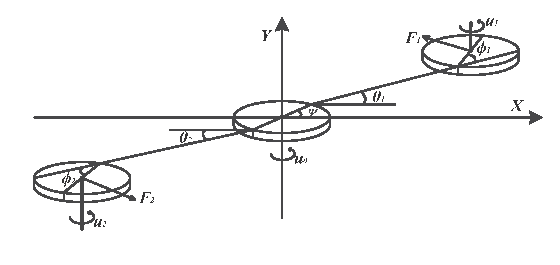
\includegraphics[width=8.91cm,height=3.91cm]{2nd_model3body.eps}
\caption{Schematic representation of three-satellite array dynamics}
\label{fig:model3body}
\end{figure}
\begin{figure}
\centering
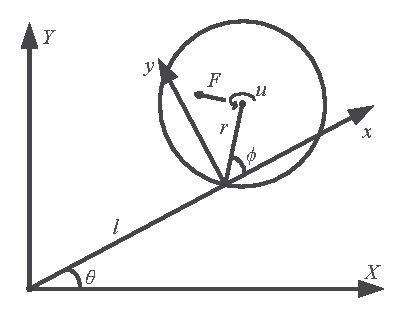
\includegraphics[width=6.46cm,height=4.82cm]{2nd_modelsinglebody.eps}
\caption{Schematic representation of single satellite dynamics}
\label{fig:modelsinglebody}
\end{figure}
To our knowledge, flywheels are applied as the proper actuators frequently in the attitude regulation of the satellite, for instance, the system of the SPECS project in an orbit around the L2 lagrange point is manoeuvred by using the flywheel control strategy in most of the time~\cite{chung2008propellant1}. The types of flywheel can be divided into the bias moment and the zero moment according to the mechanical structure. The rotation rate of the bias moment wheels is nonnegative, and the zeros moment ones can change the rotation direction. The zero moment wheels are also called the reaction wheels, which may always maintain the whole satellite's moment zero, and they are used more widely than the bias ones in the stability control of the satellite attitude. Considering the energy consumption of the system in practice, wheels are driven by electricity which may be provided by energy harvesting system, whereas the limit on the fuel, that a satellite can carry with, makes the life of the thrust control strategy shorter than the reaction wheel control. Satellites need reaction wheels to generate the continuous high precise torque for the attitude regulation in orbit; thrusters consume expensive fuel to supply the linear torque output in pulse method. In addition, the reaction wheel is convenient to equip, and there always exists a incline reaction wheel equipped as the redundancy actuator. The thruster force is crucial to deploy the satellite into specified orbit in limited time, and the reaction wheel scheme regulates the attitude of the satellite for a long time in orbit around the earth. With neglecting the thruster force input, using the reaction wheel control strategy changes the three-satellite inline frame into an underactuated system. What is more, the effect of the input for the control system is saturated, since the torque of an reaction wheel is finite. Typically, the positive and negative torques are identical, which can be expressed by the saturation function.
\begin{align}
\bar{sat}(u)=
\begin{cases}
T_p &u > T_p\\
u   &T_n\le u\le T_p\\
T_n &u < T_n
\end{cases}
\end{align}
where $T_p$ and $T_n$ denote the maximal positive and negative torque respectively. According to aforementioned analysis, the equations for the dynamics of the individual satellite shown in Fig \ref{fig:modelsinglebody} holds
\begin{align}
M_1(\phi)
\begin{pmatrix}
\ddot{\theta}\\
\ddot{\phi}
\end{pmatrix}
+C_1(\phi,\dot{\theta},\dot{\phi})
\begin{pmatrix}
\dot{\theta}\\
\dot{\phi}
\end{pmatrix}
+
\begin{bmatrix}
2m(r\cos{\phi}+l)\dot{\theta}\dot{l}\\
2mr\cos{\phi}\dot{\theta}\dot{l}
\end{bmatrix}
=
\begin{bmatrix}
1\\
1
\end{bmatrix}\bar{sat}(u)\label{eq:individualsys}
\end{align}
where $\bar{sat}()$ means the saturation characteristics. According to the zero tether speed assumption $\dot l=0$, the preceding equations coincides with Eq. (\ref{eq:3bodyreduce}). Attend to the problem of the reduced three-satellite inline tethered formation, and the following lemma is proposed to demonstrate the stability of the coupled attitude dynamics shown in Eq. (\ref{eq:3bodymodel}).
\begin{mylem}
Synchronization and Partial Contraction~\cite{wang2005partial}. Consider two nominal coupled system which have the relation
\begin{align}
\dot{x}_1-f(x_1,t)=\dot{x}_2-f(x_2,t)\notag
\end{align}
where the function $f(x,t)$ has contracting property in an input-independent matric, then the state $x_1$ and $x_2$ will approach each other in spite of the different initial requirement.\label{thm:syn}
\end{mylem}
According to Lemma \ref{thm:syn}, Eq. (\ref{eq:3bodyreduce}) indicates that the formulation of two sub-systems meets the contracting requirement, hence $(\theta_1,\phi_1)^T$ and $(\theta_1,\phi_2)^T$ will coverage to each other thereby if an individual control law is designed to guarantee the stability of the each one~\cite{huang2015nonlinear}.\par
This work ignores the linear force, and hence the system becomes underactuated and input saturated.
As $M_1(\phi)$ is invertible, select state variable $x_1=\theta$, $x_2=\dot\theta$, $x_3=\phi$, $x_4=\dot\phi$ to get the following state space equations, which express the attitude dynamics of the individual participating satellite shown in Figure \ref{fig:modelsinglebody}:
\begin{align}
\begin{split}
&\dot x_1 = x_2\\
&\dot x_2 = f_1(X,t)+d_1(X,t)+b_1(X,t)\bar{sat}(u)\\
&\dot x_3 = x_4\\
&\dot x_4 = f_2(X,t)+d_2(X,t)+b_2(X,t)\bar{sat}(u)
\end{split}\label{eq:model}
\end{align}
where $X = (x_1,x_2,x_3,x_4)^T$, and $f_1(X,t)$ and $f_2(X,t)$ are nonlinear functions:
\begin{align*}
f_1(X,t) =& \frac{I_rrl(x_2+x_4)\sin x_3+mr^2l^2x_2\cos x_3\sin x_3}{I_rl^2-mr^2l^2\cos{^2x_3}}x_2\\
          &+\frac{I_rx_4 mrl(x_2+x_4)\sin x_3 }{I_rml^2-m^2r^2l^2\cos{^2x_3}}\\
f_2(X,t) =& \frac{(I_r+mrl\cos x_3)mrlx_4\sin x_3-I_r(I_r+ml^2+2mrl\cos x_3)}{m^2r^2l^2\cos{^2x_3}-I_rml^2}x_2\\
          &+\frac{[mrl(x_2+x_4)\sin x_3](I_r+mrl\cos x_3)}{m^2r^2l^2\cos{^2x_3}-I_rml^2}x_4\\
b_1(X,t) =&-\frac{mrl\cos x_3}{I_rml^2-m^2r^2l^2\cos{^2x_3}}\\
b_2(X,t) =&\frac{mrl\cos x_3+ml^2}{I_rml^2-m^2r^2l^2\cos{^2x_3}}
\end{align*}
In addition, $d_1(X,t)$ and $d_2(X,t)$ denote the external perturbations such as the gravity gradient torque, the solar pressure torque, the aerodynamic torque or the magnetic torque, and among the previous perturbations, the aerodynamic torque is the crucial factor, which will affect the stability of the attitude dynamics.\par
In this work, the attitude regulation of the individual satellite expressed in Eq.(\ref{eq:model}), which is an underactuated and coupling input system, is achieved by utilizing the variable structure theory, with emphasis on the solution of the actuators saturation. Once the states of Eq.(\ref{eq:model}) is stable, according to Lemma \ref{thm:syn}, the entire three-satellite array can be adjusted to be a fixed-point rotation system.
\subsection{Modified Hierarchial Sliding Mode Control with Input Saturation}\label{sec:SMC}
The issue about attitude regulation of the three-satellite inline tethered system is converted into designing the independent control system for the attitude regulation of the individual satellite described as Eq. (\ref{eq:model}), and meanwhile, the system is strict saturated, coupled and nonlinear. There exists a stable hierarchial sliding mode approach (HSM) investigated for a class of second order underactuated systems, such as Acrobot, overhead crane and pendubot etc~\cite{wang2004design}, and the state space equations of the these models are similar to the form of Eq. (\ref{eq:model}). Considering the effect of the input saturation of the individual satellite, and furthermore, synthesizing the HSM and adaptive sliding mode designs derives the modified method, which can overcome both the input saturation and coupling characteristics.\par
In the symbol system of the control system, the time variable is often abbreviated if it won't lead the formulations confused, i.e., $S(t)$ may be simplified as $S$ usually. HSM structures the first-level sliding surfaces as follows:
\begin{align}
\begin{split}
s_1 = c_1x_1+x_2\\
s_2 = c_2x_3+x_4
\end{split}\label{eq:s1s2}
\end{align}
where $c_1$ and $c_2$ are suitable parameters and always positive. Construct the input to supply the convergence of the second-level sliding surface in finite time:
\begin{align}
S=\alpha s_1+\beta s_2\label{eq:S}.
\end{align}\par
The proceeding of HSM design is omitted. There is an important lemma mentioned for the modified approach design.
\begin{mylem}Hierarchical Convergence~\cite{wang2004design}.
Considering a sort of underactuated systems which own a stabel equilibrium point, propose the sliding surfaces as Eq. (\ref{eq:model}), Eq. (\ref{eq:s1s2}), Eq. (\ref{eq:S}), and there is a approach to guaranteeing the convergence of the second-level sliding mode in finite time. If $s_1\in L_\infty$, $\dot s_1\in L_\infty$, then the first-level sliding mode also converges in finite time.\label{lm:1}
\end{mylem}
Consider the nominal nonlinear system Eq. (\ref{eq:model}), and rewrite $\bar{sat}(u)$ as $\bar{sat}(u) = R(u)u$. Note that $0 \le R(u) \le 1$
\begin{equation}
R(u) =\begin{cases}
u_{max}/u   & u > u_{max}\\
1           & u_{min} \le u \le u_{max}\\
u_{min}/u   & u < u_{min}
\end{cases}
\end{equation}
where $u_{max}(u_{min})$ is the maximum torque that the reaction wheel can generate in positive (negative) direction, and there is a restriction $u_{min}<0<u_{max}$, $u_{min}=-u_{max}$ for guaranteeing the predefined condition $0<R(u)\le 1$.\par
There exist the following assumptions in this paper.
\begin{assumption}
The uncertain dynamic system with nonlinearities indicated in Eq. (\ref{eq:model}) is controllable.\label{as:1}
\end{assumption}
\begin{assumption}
$d_1(X,t)$ and $d_2(X,t)$ are the uncertain parts of system (\ref{eq:model}), and satisfies the following relation $max(\vert d_1(X,t)\vert,\vert d_2(X,t)\vert) \le \zeta <\infty$, $\zeta$ is constant positive.\label{as:2}
\end{assumption}
\begin{myrem}
The mathematical form of $d_i(X,t)$ is trigonometric term, and the detail of $d_i(X,t)$ will be given in Section \ref{sec:sm}. Assumption \ref{as:2} is reasonable since there exists the boundary of the mentioned perturbation. In addition, it is obvious that the terms in the individual satellite system (\ref{eq:3bodyreduce}) consist of the trigonometric and constant terms, and hence the extremes of $\vert c_1x_2+f_1(X,t)\vert$ and $\vert c_2x_4+f_2(X,t)\vert$ can be obtained by using mathematical calculation.
\end{myrem}
Modified hierarchical sliding mode control (MHSM) constructs the first- and second-level surfaces in the same way, thanks to the Lemma \ref{lm:1} and Assumption \ref{as:2}, we propose the adaptive control input as follows:
\begin{align}
u = -\frac{\rho\delta\eta(t)}{\alpha b_1(X,t)+\beta b_2(X,t)}sgn(S)\label{eq:u}.
\end{align}\par
In the preceding expression
\begin{align}
\rho &= 2(\alpha+\beta)max(\zeta,\vert c_1x_2+f_1(X,t)\vert,\vert c_2x_4+f_2(X,t)\vert)
\end{align}
and $\delta>1$. The derivative of $\eta(t)$ has the characteristics, $\dot{{\eta}}(t) = \rho\gamma\delta e^{-2\gamma^{-1}{\eta}^{-1}(t)}\vert S\vert$ , $\eta(0) > 0$ so that the $\eta(t)$ is constant positive. $\gamma$ is a parameter for cancelling the input saturation, and it will be discussed later on. Hence the crucial theorem is given.
\begin{thm}
The nonlinear system which can be expressed as Eq.(\ref{eq:model}), satisfies the Assumption \ref{as:1} and \ref{as:2}, and if the candidate of system input is Eq. (\ref{eq:u}), the trajectories of the system asymptotically converge to the sliding surface $S = 0$.
\end{thm}
\begin{proof}
Select the Lyapunov function candidate
\begin{equation}
V = \frac{1}{2}S^2+\frac{1}{2}v^2\label{eq:V}
\end{equation}
where $v = {\eta}(t)e^{\gamma^{-1}{\eta}^{-1}(t)}$, then introduce Eq.(\ref{eq:S}) and Eq.(\ref{eq:u}) into the derivative of $V$ to obtain
\begin{align}
\begin{split}
\dot{V} &= S\dot S+v\dot v\\
        &= S[\alpha(c_1x_2+f_1(X,t)+d_1(X,t)+b_1(X,t)\bar{sat}(u))\\
        &\quad+\beta(c_2x_3+f_2(X,t)+d_2(X,t)+b_2(X,t)\bar{sat}(u))]+v\dot v\\
        &\le \rho\vert S\vert - R(u)\rho\delta\eta(t)\vert S\vert +v\dot v\label{eq:dotV}
\end{split}
\end{align}
It is explicit to realize that $0 < R(u(t)) \le 1$, and a constant positive $\gamma$ can be selected to satisfy
\begin{equation}
0<\gamma\le R(u)\le 1 \label{eq:utl}
\end{equation}
Moreover, term $R(u)\rho\delta\eta(t)\vert S\vert$ is positive, and $0\le R(u)\le 1$. The Inequality.(\ref{eq:dotV}) becomes the interim form:
\begin{align}
\dot{V} \le \rho\vert S\vert - \rho\gamma\delta\eta(t)\vert S\vert +v\dot v\label{eq:dotVinterim}
\end{align}
Derive $v\dot v$ as follows
\begin{align}
\begin{split}
v\dot v &= \dot{\eta}e^{2\gamma^{-1}\eta^{-1}(t)}(\eta(t)-\gamma^{-1})\\
        &= \rho\gamma\delta(\eta(t)-\gamma^{-1})\vert S\vert\label{eq:vdotv}
\end{split}
\end{align}
Substitute Eq.(\ref{eq:vdotv}) into Eq.(\ref{eq:dotVinterim}), and yield
\begin{align}
\dot{V} \le (1 -\delta)\rho\vert S\vert\le 0 \label{eq:dotVfinal}
\end{align}
$\dot{V}$ is negative semi-definite while $V$ is positive definite, and moreover, bounded functions $S$ and ${\eta}(t)$ ensure that $\lim\limits_{t\to\infty}V$ exists. Inequality.(\ref{eq:dotVfinal}) can be integrated
\begin{align}
\begin{split}
V(0) &\ge V(t) + \int_{0}^{t}(\delta-1)\rho\vert S(\tau)\vert d\tau\\
&\ge \int_{0}^{t}(\delta-1)\rho\vert S(\tau)\vert d\tau\label{eq:V10}
\end{split}
\end{align}
According to the description of Barbalat's lemmas, $t\to\infty$ implies $S(t)\to 0$. Hence, proof is demonstrated completely.
\end{proof}
\section{Adaptive Sliding Control For Two-satellite Array System}\label{sec:SMC2}
The three-satellite inline array can be simplified as three individual satellite systems by above-mentioned model reduction technology, and in this section, a two-satellite array system shown in Figure \ref{fig:model2body} is investigated, in which two satellites are the participants connected with a stiff space tether. The dynamic equations of the two-satellite array system can be described as follows:
\begin{figure}[H]
\centering
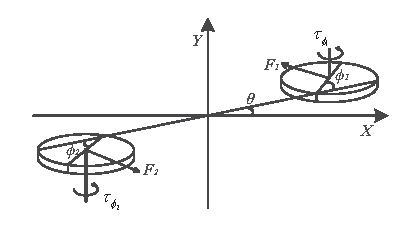
\includegraphics[width=6.30cm,height=3.29cm]{2nd_model2body.eps}
\caption{Schematic representation of two-satellite system dynamics}
\label{fig:model2body}
\end{figure}
\begin{align}
M_3(\phi_1,\phi_2)
\begin{pmatrix}
\ddot{\theta}\\
\ddot{\phi}_1\\
\ddot{\phi}_2
\end{pmatrix}
+C_5(\phi_1,\phi_2,\dot{\theta},\dot{\phi}_1,\dot{\phi}_2)
\begin{pmatrix}
\dot{\theta}\\
\dot{\phi}_1\\
\dot{\phi}_2
\end{pmatrix}
+
\begin{pmatrix}
2m(r\cos\phi_1+r\cos\phi_2+2l)\dot\theta\dot l\\
2mr\cos\phi_1\dot\theta\dot l\\
2mr\cos\phi_2\dot\theta\dot l
\end{pmatrix}
=
\begin{pmatrix}
\tau_{\phi_1}+\tau_{\phi_2}\\
\tau_{\phi_1}\\
\tau_{\phi_2}
\end{pmatrix}\label{eq:2body}
\end{align}
where
\begin{align}
&M_3(\phi_1,\phi_2)
=\begin{bmatrix}
m_{11}(\phi_1)+m_{11}(\phi_2) &m_{12}(\phi_1) &m_{12}(\phi_2)\\
m_{21}(\phi_1) &m_{22} &0\\
m_{21}(\phi_2) &0      &m_{22}
\end{bmatrix}\label{eq:M3}\\
&C_5(\phi_1,\phi_2,\dot{\theta},\dot{\phi}_1,\dot{\phi}_2)
=\begin{bmatrix}
c_{11}(\phi_1,\dot{\phi}_1)+c_{11}(\phi_2,\dot{\phi}_2) &c_{12}(\phi_1,\dot{\theta},\dot{\phi}_1) &c_{12}(\phi_2,\dot{\theta},\dot{\phi}_2)\\
c_{21}(\phi_1,\dot{\theta}) &c_{22} &0\\
c_{21}(\phi_2,\dot{\theta}) &0 &c_{22}
\end{bmatrix}\label{eq:C5}
\end{align}
and the elements $m_{11}=m_{12}$, $m_{22}$, $m_{21}$, $c_{11}$, $c_{12}$, $c_{21}$ and $c_{22}$ in Eq. (\ref{eq:M3}) and Eq. (\ref{eq:C5}) are defined in the attitude dynamics of the individual satellite in Eq. (\ref{eq:M1}) and Eq. (\ref{eq:C1}).\par
Compared to the three-satellite inline array, the central satellite is absent in the two-satellite system so that the individual torque acting on one participant will effect the other one~\cite{chung2007nonlinear}. With model reduction technology failing in the two-satellite system, the systemical simplification is unable to be achieved, due to the fact that the physical construction of the satellite is almost identical, and the participating satellite having the same mechanical structure results in that the two-satellite system do not satisfy the condition of station keeping like the simple mother satellite and sub-satellite tethered system. In the mother satellite and sub-satellite tethered system, it requires the mass of one satellite to be much larger than the other one, and this premise of assumption is usually met in the deployment mission of the tethered satellite system. Without any simplification, the number of the input in Eq. (\ref{eq:2body}) is less than the degree of freedom (DOF), and meanwhile the input is coupled as well. In addition, the condition of the actuator is same to the three-satellite inline array, which means that the flywheel is the only actuator for attitude regulation of the satellite. According to the previous results, two-satellite inline system is underactuated and coupled input saturated.\par
The solution for the attitude stability of the three-satellite inline array is valid for the two-satellite inline system. For the sake of the adaptive controller design, the system can be rewritten as the expression of Eq. (\ref{eq:model}). As $M_3(\phi_1,\phi_2)$ is invertible, select state variables $x_1=\theta$, $x_2=\dot\theta$, $x_3=\phi_1$, $x_4=\dot\phi_1$, $x_5=\phi_2$, $x_6=\dot\phi_2$ to get the following state space equations:
\begin{align}
\begin{split}
&\dot x_1 = x_2\\
&\dot x_2 = f_1(X,t)+d_1(X,t)+b_1(X,t)\bar{sat}(u_1)+b_2(X,t)\bar{sat}(u_2)\\
&\dot x_3 = x_4\\
&\dot x_4 = f_2(X,t)+d_2(X,t)+b_3(X,t)\bar{sat}(u_1)+b_4(X,t)\bar{sat}(u_2)\\
&\dot x_5 = x_6\\
&\dot x_6 = f_3(X,t)+d_3(X,t)+b_5(X,t)\bar{sat}(u_1)+b_6(X,t)\bar{sat}(u_2)
\end{split}\label{eq:2model}
\end{align}
where $X = (x_1,x_2,x_3,x_4,x_5,x_6)^T$. In addition, $\bar{sat}()$, $f_i(X,t)$ and $d_i(X,t)$ have the similar mathematical feature which is illustrated in the individual system of three-satellite inline array in Eq. (\ref{eq:model}), and $f_i(X,t)$ and $b_i(X,t)$ can be derived:
\begin{align}
\begin{split}
\begin{pmatrix}
f_1(X,t)\\
f_2(X,t)\\
f_3(X,t)
\end{pmatrix}=
M_3^{-1}(x_3,x_5)C_5(x_3,x_5,x_2,x_4,x_6)
\begin{pmatrix}
x_2\\
x_4\\
x_6
\end{pmatrix}
\end{split}
\end{align}
\begin{align}
\begin{split}
\begin{pmatrix}
b_1(X,t)&b_2(X,t)\\
b_3(X,t)&b_4(X,t)\\
b_5(X,t)&b_6(X,t)
\end{pmatrix}=
M_3^{-1}(x_3,x_5)
\begin{pmatrix}
1 &1\\
1 &0\\
0 &1
\end{pmatrix}
\end{split}
\end{align}
where $M_3^{-1}(x_3,x_5)$ is the inverse matrix of $M_3(x_3,x_5)$:
\begin{footnotesize}
\begin{align*}
&M_3^{-1}(x_3,x_5)
=\frac{\begin{bmatrix}
m_{22}^2 &-m_{12}(x_3)m_{22} &m_{22}m_{12}(x_5)\\
-m_{22}m_{21}(x_3) &[m_{11}(x_3)+m_{11}(x_5)]m_{22}-m_{12}^2(x_5) &m_{12}(x_5)m_{21}(x_3)\\
-m_{22}m_{21}(x_5) &m_{12}(x_3)m_{21}(x_5) &[m_{11}(x_3)+m_{11}(x_5)]m_{22}-m_{12}^2(x_3)
\end{bmatrix}}{[m_{11}(x_3)+m_{11}(x_5)]m_{22}^2-m_{12}(x_5)m_{21}(x_5)m_{22}-m_{12}(x_3)m_{21}(x_3)m_{22}}\\
&=\frac{\begin{bmatrix}
I_r^2 &-I_r(I_r+mrl\cos\phi_1) &-I_r(I_r+mrl\cos\phi_2)\\
-I_r(I_r+mrl\cos\phi_1) &I_r(I_r+2ml^2+2mrl\cos\phi_1)-m^2r^2l^2\cos^2\phi_2 &(I_r+mrl\cos\phi_2)(I_r+mrl\cos\phi_1)\\
-I_r(I_r+mrl\cos\phi_2) &(I_r+mrl\cos\phi_2)(I_r+mrl\cos\phi_1) &I_r(I_r+2ml^2+2mrl\cos\phi_2)-m^2r^2l^2\cos^2\phi_1
\end{bmatrix}}{I_rml^2(2I_r-mr^2\cos{^2\phi_1}-mr^2\cos{^2\phi_2})}.
\end{align*}
\end{footnotesize}\par
For proceeding to apply the MHSM control to the attitude regulation of the two-satellite inline system shown in Eq. (\ref{eq:2model}), the first-level iedal sliding surfaces are selected firstly as follows:
\begin{align}
\begin{split}
\sigma_1 = \bar{c}_1x_1+x_2\\
\sigma_2 = \bar{c}_2x_3+x_4\\
\sigma_3 = \bar{c}_3x_4+x_5
\end{split}\label{eq:sigma123}
\end{align}
where $\bar{c}_i$ is the suitable positive coefficient, and the second sliding surface follows:
\begin{align}
\bar{S} = \bar{\alpha}\sigma_1+ \bar{\beta}\sigma_2+\bar{\iota}\sigma_3\label{eq:bar S}
\end{align}
where $\bar{\alpha}$, $\bar{\beta}$ and $\bar{\iota}$ are positive coefficients.
\begin{myrem}
Some essential results are given in advance so that the adaptive control design for the system in Eq. (\ref{eq:2model}) can be illustrated explicitly. The spatial perturbation term, $d_i(X,t)$, owns the characteristics of trigonometric function, and those bound value can be determined easily. It is noted that the terms in the attitude dynamics of the two-satellite system in Eq. (\ref{eq:2body}) are a group of constant and trigonometrical terms, and in addition, their operations are additive and multiplicative. Hence the boundary exists and can be calculated. In the process of the attitude regulation, the attitude angle is limited in a practical meaningful range $\vert \phi_i\vert<\pi/2$~\cite{chung2008propellant2}. Therefore, some symbols are introduced to express the mentioned relationship, and they will take part in the design of the adaptive control in the following form:\label{rem:2}
\begin{align}
\begin{split}
\bar\varpi &\ge \max(\vert d_1(X,t)\vert,\vert d_2(X,t)\vert,\vert d_3(X,t)\vert)\\
\bar\xi &=  \max(\vert \bar c_1x_2 + f_1(X,t)\vert,\vert \bar c_2x_4 + f_2(X,t)\vert,\vert \bar c_3x_6 + f_3(X,t)\vert)
\end{split}
\end{align}
\end{myrem}
The adaptive control inputs for stabilizing the attitude dynamics of the two-satellite system in Eq. (\ref{eq:2model}) are given directly:
\begin{align}
\begin{split}
u_1 = -\frac{\bar\delta\bar\rho\eta_1(t)sgn(\bar S)+k_1\bar S}{\bar\alpha b_1(X,t) + \bar\beta b_3(X,t) + \bar\iota b_5(X,t)}\\
u_2 = -\frac{\bar\delta\bar\rho\eta_2(t)sgn(\bar S)+k_2\bar S}{\bar\alpha b_2(X,t) + \bar\beta b_4(X,t) + \bar\iota b_6(X,t)}.
\end{split}\label{eq:u1u2}
\end{align}\par
In preceding equation
\begin{align}
\bar\rho &\ge 2(\bar\alpha + \bar\beta + \bar\iota)\max(\bar\varpi,\bar\xi)
\end{align}
and $\bar\eta(t)=\eta_1(t)+\eta_2(t)$ whose derivative has the characteristics, $\dot{{\bar\eta}}(t) = \bar\rho\bar\gamma\bar\delta e^{-2\bar\gamma^{-1}{\bar\eta}^{-1}(t)}\vert \bar S\vert$ , $\bar\eta(0) > 0$ so that the $\bar\eta(t)$ is a positive constant. $k_1+k_2\ge 0$, $\bar\delta >1$, and in addition, the input saturation can be described by $\bar{sat}(u_i) = R(u_i)u_i, i =1,2$, whose bound of $R(u_i)$ has the characteristics, $0<\bar\gamma\le \min(R(u_1),R(u_2))\le 1$. The crucial theorem follows.
\begin{thm}
Considerinig the nonlinear system which is shown as Eq. (\ref{eq:2model}) and the constraint conditions of the system established in Remark \ref{rem:2}, if the candidate of the system inputs are expressed as Eq. (\ref{eq:u1u2}), the trajectories of the system will asymptotically converge to the ideal sliding surface $\bar S=0$.\label{thm:3}
\end{thm}
\begin{proof}
Select the Lyapunov function candidate
\begin{align}
\bar V = \frac{1}{2}\bar S^2 + \frac{1}{2}\bar v^2
\end{align}
where $\bar v = {\bar\eta}(t)e^{\bar\gamma^{-1}{\bar\eta}^{-1}(t)}$, then introduce Eq.~(\ref{eq:bar S}) and Eq.~(\ref{eq:u1u2}) into the derivative of $V$ to obtain
\begin{align}
\begin{split}
\dot{\bar V} &= \bar{S}\dot{\bar{S}}+\bar v\dot{\bar v}\\
                &= \bar{S}(\bar\alpha[\bar c_1 x_2 + f_1(X,t) + d_1(X,t) + b_1(X,t)\bar{sat}(u_1) + b_2(X,t)\bar{sat}(u_2)]\\
                     &\quad+         \bar\beta [\bar c_2 x_4 + f_2(X,t) + d_2(X,t) + b_3(X,t)\bar{sat}(u_1) + b_4(X,t)\bar{sat}(u_2)]\\
                     &\quad+         \bar\iota[\bar c_3 x_6 + f_3(X,t) + d_3(X,t) + b_5(X,t)\bar{sat}(u_1) + b_6(X,t)\bar{sat}(u_2)])+\bar v\dot{\bar v}\\
                     &\le \bar\rho\vert\bar S\vert + \bar S[(\bar\alpha b_1(X,t) + \bar\beta b_3(X,t) + \bar\iota b_5(X,t))R(u_1)u_1\\
                     &\quad+(\bar\alpha b_2(X,t) + \bar\beta b_4(X,t) + \bar\iota b_6(X,t))R(u_2)u_2]+\bar v\dot{\bar v}\\
                     &\le \bar\rho\vert\bar S\vert - \bar S[ R(u_1)(\bar\delta\bar\rho\eta_1(t)sgn(\bar S)+k_1\bar S)+R(u_2)(\bar\delta\bar\rho\eta_2(t)sgn(\bar S)+k_2\bar S)]+\bar v\dot{\bar v}\\
                     &\le \bar\rho\vert\bar S\vert - \gamma(k_1+k_2)\bar S^2 - \bar\delta\bar\rho\bar\gamma\bar\eta(t)\vert\bar S\vert+\bar v\dot{\bar v}.
\end{split}
\end{align}\par
Referring to Eq.(\ref{eq:vdotv}), above expression can be derived to
\begin{align}
\dot{\bar V} \le (1 -\bar\delta)\bar\rho\vert\bar S\vert- \bar\gamma(k_1+k_2)\bar S^2\le 0 .\label{eq:dotbarVfinal}
\end{align}\par
According to the description of Barbalat's lemmas and referring to Eq.~(\ref{eq:V10}), $t\to\infty$ implies $S(t)\to 0$. Hence the second-level sliding surface in Eq.~(\ref{eq:bar S}) is stable, and proof is demonstrated completely.
\end{proof}
\begin{myrem}
Theorem \ref{thm:3} is proposed for guaranteeing that the sliding mode dynamics will reach the ideal surface $\bar S$ in finite time, and the adaptive update ${\bar\eta}(t)$ eliminate the effect of the input saturation in the two-satellite system. Moreover, considering the convergence of the first-level sliding mode dynamics, and according to the article~\cite{wang2004design}, they are asymptotically stable, and the proof is omitted here.
\end{myrem}
\section{Numerical Simulation}\label{sec:sm}
For exhibiting the effectiveness of the proposed control schemes designed for the multi-satellite tethered systems, numerical simulation is implemented in this section  and furthermore the analysis of simulation result verifies the preceding design in Section~\ref{sec:SMC} and Section \ref{sec:SMC2}.\par
\begin{table}[h]
\begin{center}
\caption{SPHERES properties}\label{ta:properites}
\begin{tabular}{lc}
\toprule
Properties              &RWA equiped\\
\midrule
Diameter   &0.25 m\\
Mass       &15.856 kg\\
Moment of inertia        &0.178kg$\cdot m^2$\\
Max torque actuation   &0.207Nm\\
\bottomrule
\end{tabular}
\end{center}\label{tab:1}
\end{table}
Referring to the experiment of SPHERES project, the simulation parameters describing the physical characteristics of the satellite are listed in Table \ref{tab:1}. According to the parameter list, the input boundary is determined as $T_p = -T_n = 0.207Nm$. In particular the controller's output is programmed to satisfy the restriction of the actuator, which can avoid the block of the flywheels in some extent. The length of the tether is constant, since the existence of length rate leads to an extremely complicated and unstable multi-satellite tethered systems. The reasonable length of the tether is essential, $l = 0.9m$, $\dot{l}=0m/s$, although the length will not take an important role in the following process of validating. In this simulation, it is assumed that the satellites expose itself to the real space, and there exist the solar radiation pressure torque and aerodynamic torque effecting its attitude stability in the space environment. The values of the perturbation torques are approximate to $1e^{-5}Nm$ on account of the researches on perturbation in space, and hence the external perturbation term can be expressed by a sinusoidal function whose amplitude equals to the boundary of perturbations~\cite{liu2013calculation}. Since the relative distance among the participating satellites is not large, without loss of generality, the form of preceding perturbation is identical.
\begin{align}
d_i(X,t) \approx 1e^{-5}\sin{(0.01\pi t)}\notag
\end{align}
\subsection{Individual System of Three-satellite Inline Array}
In order to apply the MHSM scheme, which is proposed in Section \ref{sec:SMC}, the parameters of the controller design is exhibited, $c_1 = 10$ and $c_2 = 3$, which meet the demand of Eq.(\ref{eq:s1s2}), the parameters of second-level sliding surface in Eq.~(\ref{eq:S}), $\alpha=\beta=1$. The adaptive parameters can be decided: $\delta = 1.8$, $\eta(0) = 1e^{-4}$, $\zeta = 1$ and $\gamma = 1e^{-4}$. $\rho$ obtained due to the simulation process, which satisfies the conditions of the finite-time convergence theory and Lyapunov stability.\par
\begin{figure}[H]
\centering
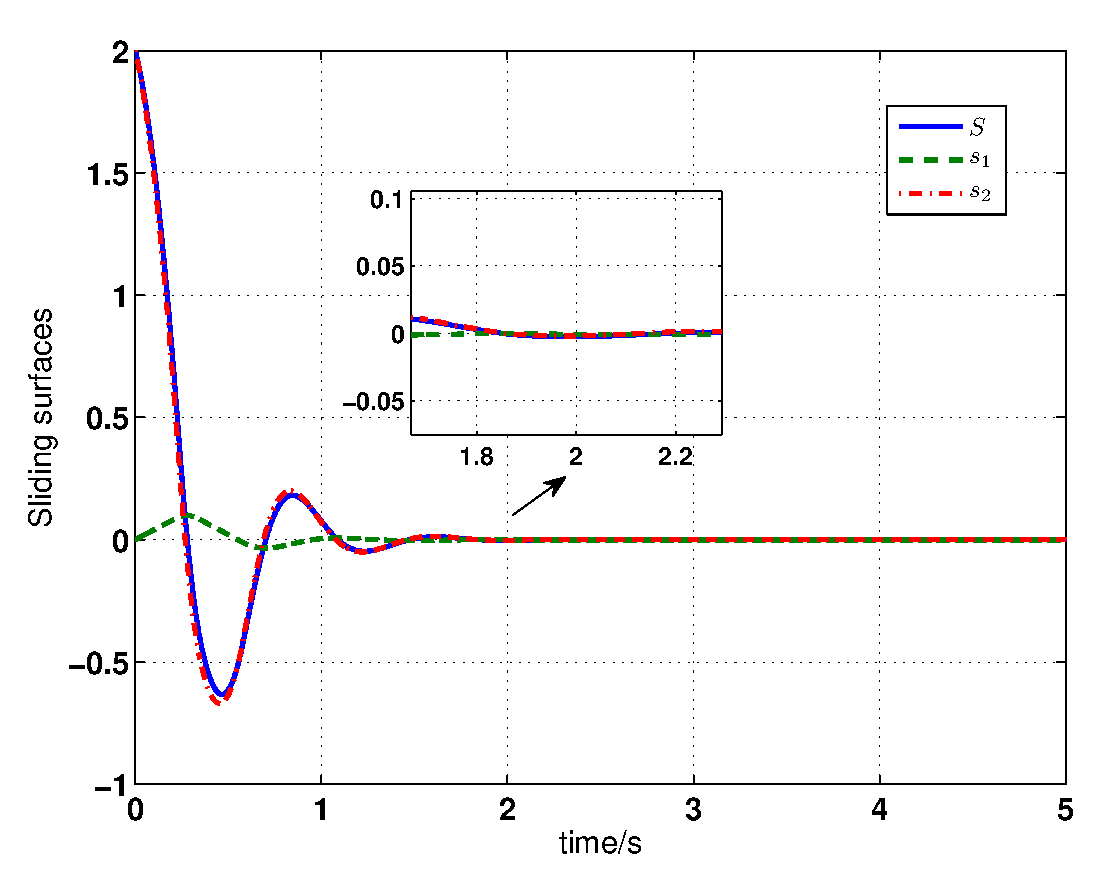
\includegraphics[width=225pt,height=180pt]{2nd_1_s.eps}
\caption{Three-satellite inline array: curves of al sliding planes}
\label{fig:sm}
\end{figure}
\begin{figure}[H]
\centering
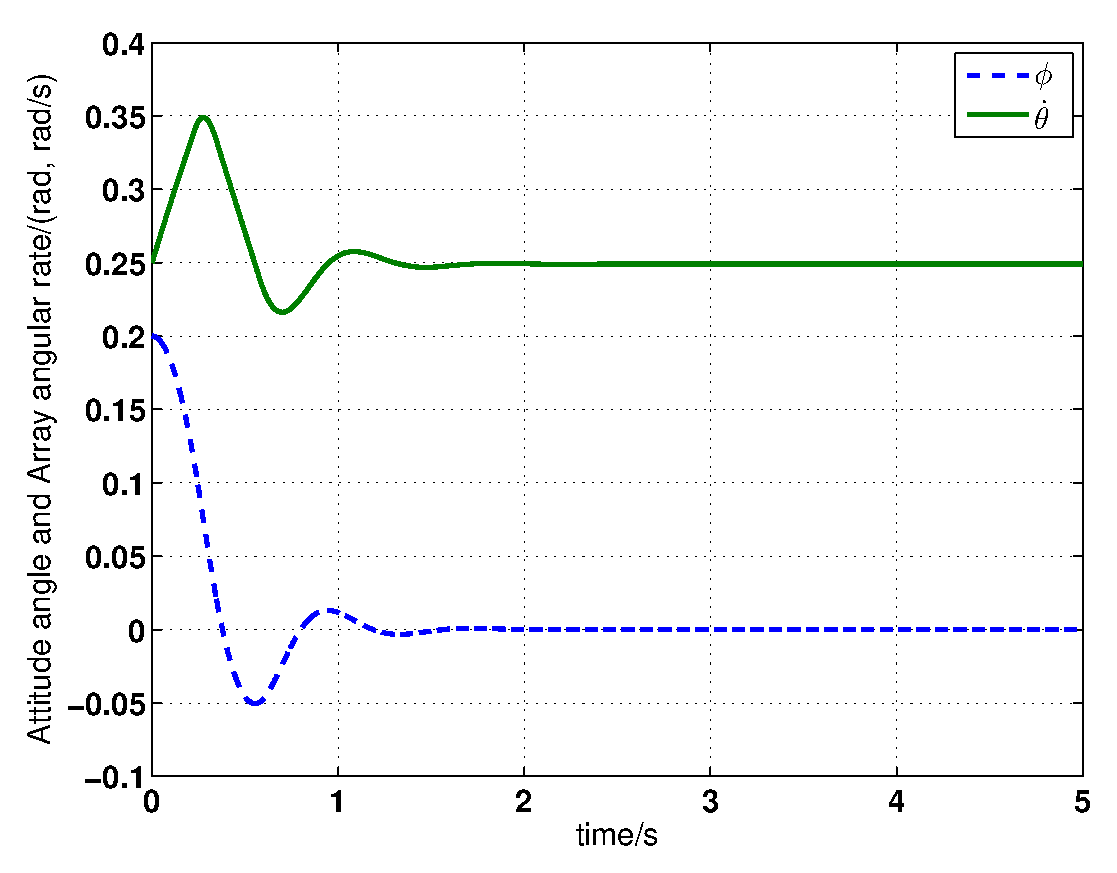
\includegraphics[width=225pt,height=180pt]{2nd_1_angle.eps}
\caption{Three-satellite inline array: attitude angle and array angular rate}
\label{fig:attitude}
\end{figure}
\begin{figure}[H]
\centering
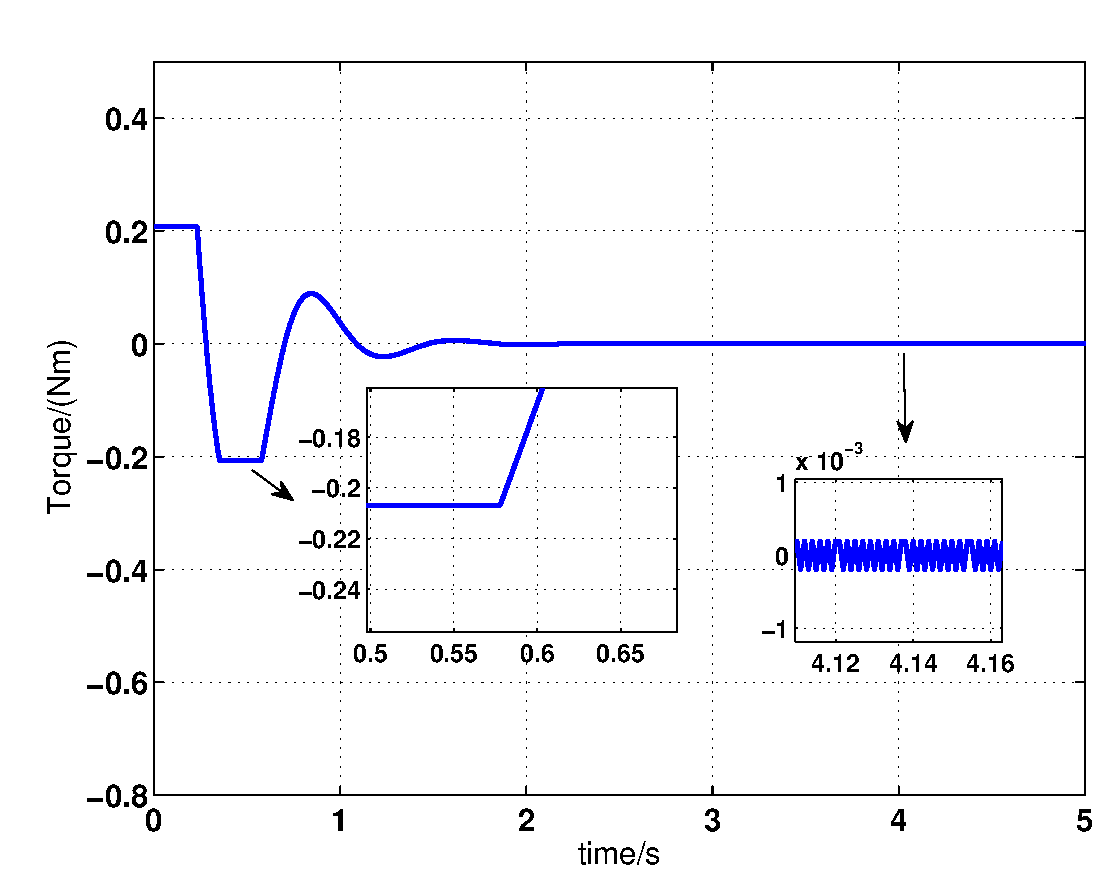
\includegraphics[width=225pt,height=180pt]{2nd_1_u.eps}
\caption{Three-satellite inline array: control torque of MHSM}
\label{fig:Torque}
\end{figure}
In this simulation, the three-satellite inline tethered system maintains rotating at angular rate $\omega_0=0.25$ in initial stage, and meanwhile, the initial individual angle, $\phi_0 = 0.25$, means that the individual system has been swung to a undesired attitude. The MHSM scheme aims to adjust the system to a desired attitude in the specified condition, and in particular the desired conditions are as follows, $\omega_d = 0.25$, $\phi_d = 0$ and $\dot{\phi}_d = 0$. In final stage, the entire three-satellite inline tethered system will keep rotating, and meanwhile three individual satellites are nonskew and in a line consequently.\par
Use MHSM scheme to regulate the individual system shown as Eq.~(\ref{eq:individualsys}), and the guidance situation of sliding mode is illustrated in Figure \ref{fig:sm} where $s_1$ and $s_2$ converge in finite time as well as $S$. It is the trajectory of $s_1$ that nearly overlaps with the one of $S$, and $s_2$ fluctuates slightly in a certain neighbour region around the origin. Paying attention on validating the convergence of each sliding mode, it is obvious that $S$, $s_1$ and $s_2$ reach the neighbour region around the origin at about $2s$ and stay stable. Furthermore, the state of the angle and the torque are both physical meaningful.\par
The situation of the attitude regulation is illustrated in Figure~\ref{fig:attitude}, in which the array angular rate is adjusted to be the desired value from the initial condition so that the individual satellites and the central satellite are rotating together at the same velocity. It is at about $2s$ when the trajectory of the attitude angle converges to the preset value, $\phi_d = 0$, so does the array angular rate.\par
The characteristics of the input saturation are exhibited in Figure~\ref{fig:Torque}, and the existence of the input bound makes the curves not smooth any more. In particular, it cuts off the oversize input signal to be a bounded value, and resume the regular input once the control signal is located in the region $[T_n,T_p]$. The bound of the input is decided by the physical property of the flywheel equipped in the satellite, and the boundary value is $0.207Nm$ bidirectionally in this section. In Figure~\ref{fig:Torque}, the saturation occurs at about $0.25s$ and $0.53s$, which is zoomed out for examining more details, and the torque keeps a low-amplitude fluctuation in the neighbour region of the origin after $2s$. That means that the torque utilized to make the system stable, still performs accurately, although the stability of the attitude dynamics for the individual satellite has achieved macroscopically. It is also easy to find that the perturbations don't introduce distinct contaminations into the control system, in another word, the anti-interference ability of the proposed scheme is excellent.
\subsection{Two-satellite System}
The parameter set of the MHSM scheme is given firstly for stabilizing the attitude of the two-satellite system expressed in Eq.~(\ref{eq:2model}) in Section~ \ref{sec:SMC2}. The parameters for first-level sliding surface design, $\bar c_1 = 5$, $\bar c_2 =3$ and $\bar c_3=1$, satisfy the positive requirement, and meanwhile, for the the second-level sliding surface design $\bar\alpha$$=\bar\beta=\bar\iota=1$ will not effect the performance of the control system in some extent. List adaptive parameters as follows: $\bar\delta = 2.1$, $\bar\eta(0)=5e^{-4}$, $\bar\gamma = 1e^{-4}$ and $\bar\varpi = 2$. In addition, $\bar\xi,\bar\rho$ can be obtained due to the simulation process. All mentioned parameters guarantee the convergence and Lyapunov stability of the system dynamics.\par
\begin{figure}[H]
\centering
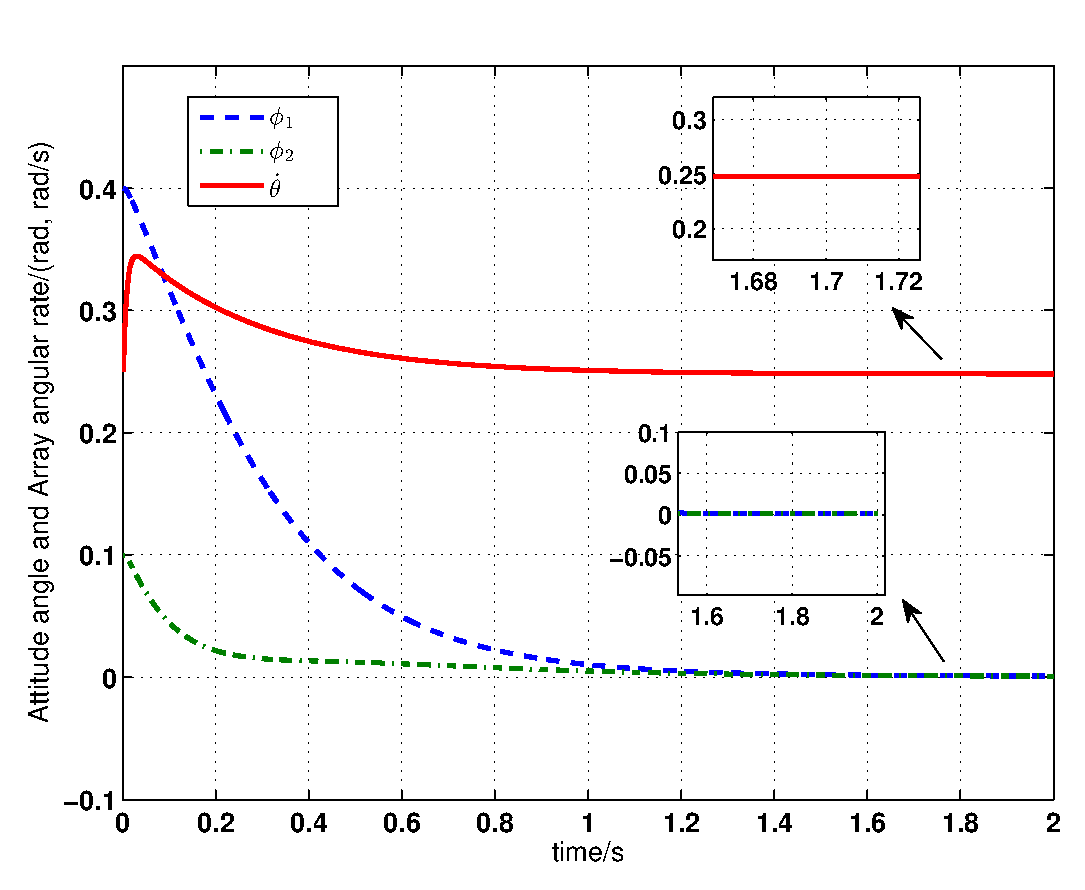
\includegraphics[width=225pt,height=180pt]{2nd_2_angle.eps}
\caption{Two-satellite system: attitude angle and array angular rate}
\label{fig:2attitude}
\end{figure}

\begin{figure}[H]
\centering
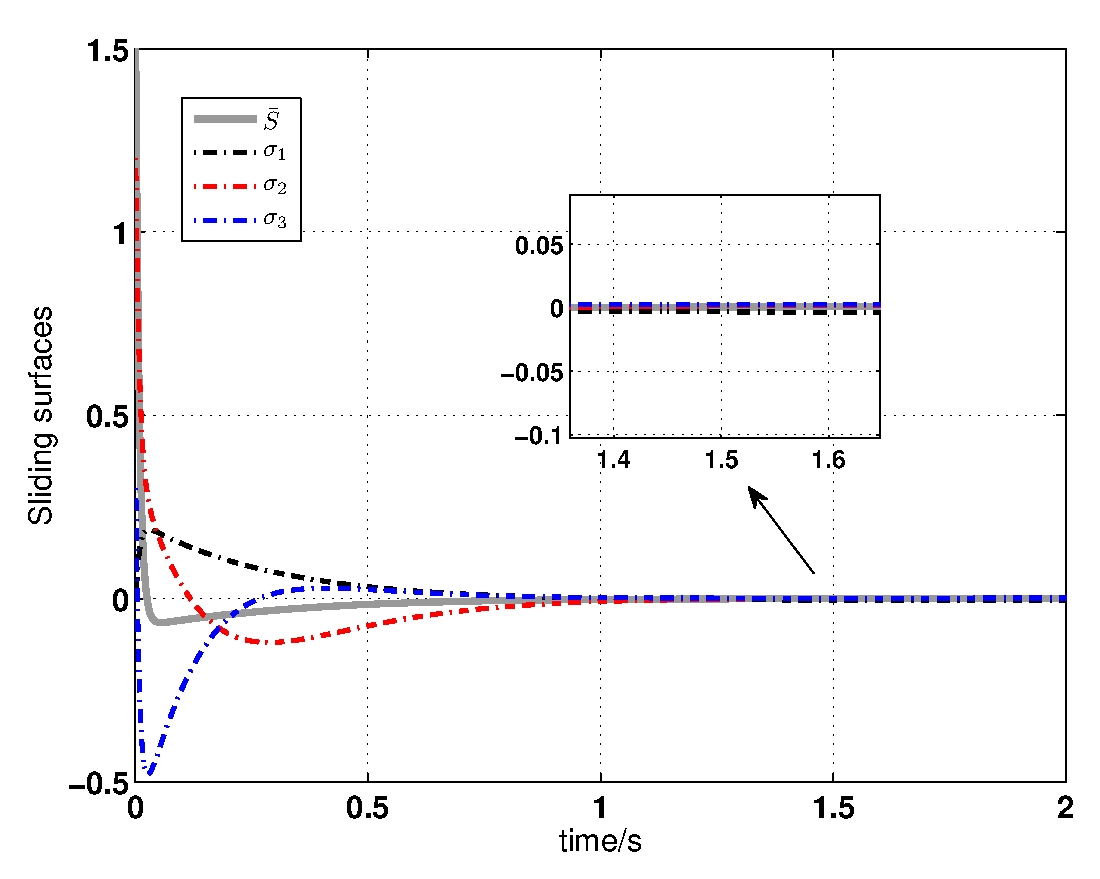
\includegraphics[width=225pt,height=180pt]{2nd_2_s.eps}
\caption{Two-satellite system: curves of all sliding planes}
\label{fig:2s}
\end{figure}

\begin{figure}[H]
\centering
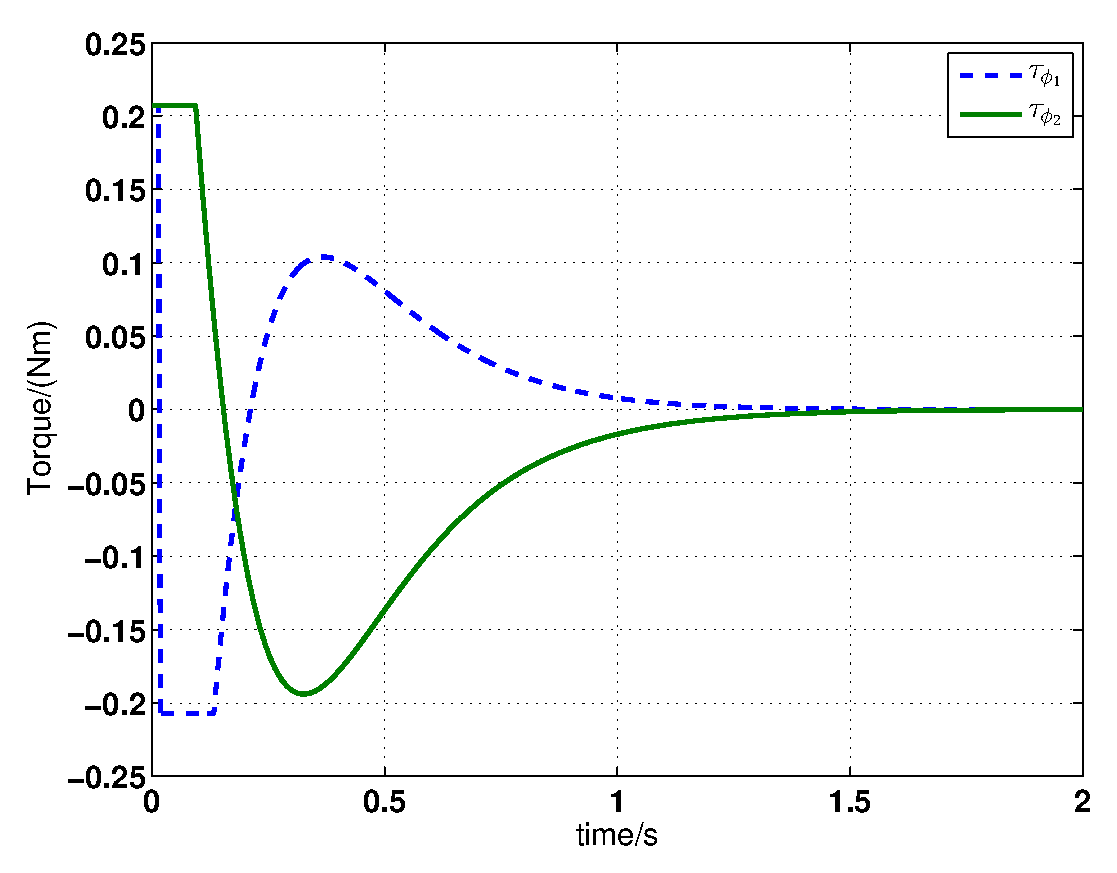
\includegraphics[width=225pt,height=180pt]{2nd_2_u1u2.eps}
\caption{Two-satellite system: control torques of MHSM}
\label{fig:2u1u2}
\end{figure}
In this part, the system is fixed-point rotating at the desired angular rate $\dot\theta_d = 0.25$, while the tether keeps stiff. In the final stage, $\phi_{i}$, the attitude angle, should be regulated to be 0.  Initially, the system rotates at the angular rate $\dot\theta_0=0.25$, and the attitude can be described by $\phi_{10}=0.4$ and $\phi_{20}=0.1$.\par
The performance of the attitude regulation can be viewed from Figure~\ref{fig:2attitude}. It shows that the angular rate of the entire system is stable at the desired rate $\dot\theta=0.25$, and meanwhile, the attitude of the participating satellites is adjusted to the desired status at about $1.8s$. Figure~ \ref{fig:2s} illustrates the guidance situation of the sliding mode, which indicates that $\sigma_i,i=1,2,3$ and $\bar S$ all converge in finite time, and then stay in the neighbour region of the origin in the subsequent time. It is noted that the first-level sliding surfaces are stable in the same time, and furthermore this phenomenon proceeds to verify Theorem \ref{thm:3}. Figure \ref{fig:2u1u2} exhibits the torques of the flywheels equipped in the participating satellites. According to the saturation characteristics of actuators, there exists the bounds of the inputs in the positive and negative direction, and the bounded inputs can be found at about $0.1s$ in this figure.
\section{Conclusion}\label{sec:Conclusion}
This paper proposes a torque control scheme to adjust the attitude of the multi-satellite array system during orbiting. In particular, the proposed approach accounts for two meaningful issues in practical implementation. The first issue is that the attitude dynamics of the multi-satellite array system is coupled and underactuated during the regulation process. The second one is that the actuators are usually saturated or bounded in the realistic application. For solving underactuated problems, the adaptive rate and the HSM control law are synthesized to obtain the MHSM control scheme, and it also takes into consideration the input saturation. The adaptive rate term is designed to compensate the impact of the saturated input so that the Lyapunov stability of the attitude dynamics can be obtained. Theoretical analysis is demonstrated to guarantee that the sliding mode dynamics reaches the ideal sliding surface in finite time and stays stability. The simulation results indicate that the attitude regulation for the tethered satellite system with the control scheme effectively and efficiently.
%Theoretical analysis is exhibited to guarantee that the states of inline tethered system reach the desired sliding mode in finite time and stay stability. The simulation results indicate that the regulating mission with the control scheme effectively and efficiently.
%The MHSM  control laws have been proposed for the attitude adjusting of multi-satellite tethered system in this paper. The procedure of control design considering  Theoretical analysis is exhibited to guarantee that the states of inline tethered system reach the desired sliding mode in finite time and stay stability. The simulation results indicate that the regulating mission with the control scheme effectively and efficiently. In addition,
\section{Acknowledgment}
This work is partially supported by the National Natural Science Foundation of China (No. 61104112, 61503097).
\section{References}
\bibliography{refdatabase}
\bibliographystyle{elsarticle-num}
%\end{twocolumn}
\end{document}
